%TC: macro \marginfootnote [other]
%TC: envir SCfigure [] other
%TC: macrocount beginSCfigure [figure]
\documentclass[11pt,twoside]{report}
\usepackage{preamble}
\setcounter{chapter}{0}
\graphicspath{{../img/}}
\def\includebibliography{}

\begin{document}
\chapter{Introduction}

\section{Overview}

%Begin with a short (1–2 pages) broader introduction for a general audience: one that my mother could understand so she knows what I’ve been working on all these years.

What precisely is covered by soft matter, and how to properly demarcate, is a matter of some academic debate.
In some sense soft matter can be most easily understood by : it is the science of ``squishy'' things.
The eminent soft matter physicist Wilson Poon describes soft matter as ``liquids with bits'' in them.
A more precise and scientific definition posits that the energy scale is subject to thermal fluctuations.
So e.g.\ chemical bonds break and reform allowing flow, but the physical processes may be arbitrarily more complex than simple liquids.

Soft matter was clearly preceded by liquids, and it is up to the individual whether liquids should be considered as the antecedent to or subsumed by soft matter.
My personal bias is that liquids represent a subset of soft matter, the zeroth order approximation to real systems.

\section{Simple liquids}

Physics is filled with toy models.
The Ising model is the most widely studied magnetic model, and the usual starting point for students learning statistical mechanics/phase transitions particular the critical point where this is \emph{the} model system.

What are simple liquids, with hard spheres at the forefront.
\hl{Hard spheres serve as a good touchstone for some of the fundamental knowns and controversies in liquid state theory and, by extension, soft matter.}
The physicists favourite toy model is the hard sphere liquid.
Interaction potential is the no-overlap condition%
\marginfootnote{I like to imagine them as ideal billiard balls, i.e.\ without any dissipative forces like friction so they continue to bounce off one another forever.}:
\begin{equation}
  U =
  \begin{cases}
    \infty & \; r < \sigma \\
    0 & \; \textrm{otherwise}.
  \end{cases}
\end{equation}
As the potential is everywhere zero or divergent, temperature has no effect on the interactions making this system athermal.
Instead, the natural control parameter is (number) density $\rho = N/V$, or as it is normally rescaled into volume fraction: the volume of space occupied by the spheres i.e.\
\begin{equation}
  \eta = \frac{N v}{V} = \rho v
\end{equation}
where $v$ is the volume of a single hard sphere.

When van der Waals wrote down their famous equation of state for real gases, i.e.\
\begin{equation}
  (p - a N)(V - Nv) = N k_B T
\end{equation}
where $V - Nv$ corrects for the volume occupied by finite-sized particles and $p - aN$ for the interactions,
it was widely believed that to go beyond this to understand liquids more sophisticated treatments of the \emph{attractions} would be required.
History shows that in actual fact the treatment of \emph{repulsions} were lacking.
It turns out that to a large degree simple liquids can be considered as hard spheres plus an attractive perturbation: an accurate treatment of the repulsion is needed, attractions can be less accurate.

\begin{SCfigure}
  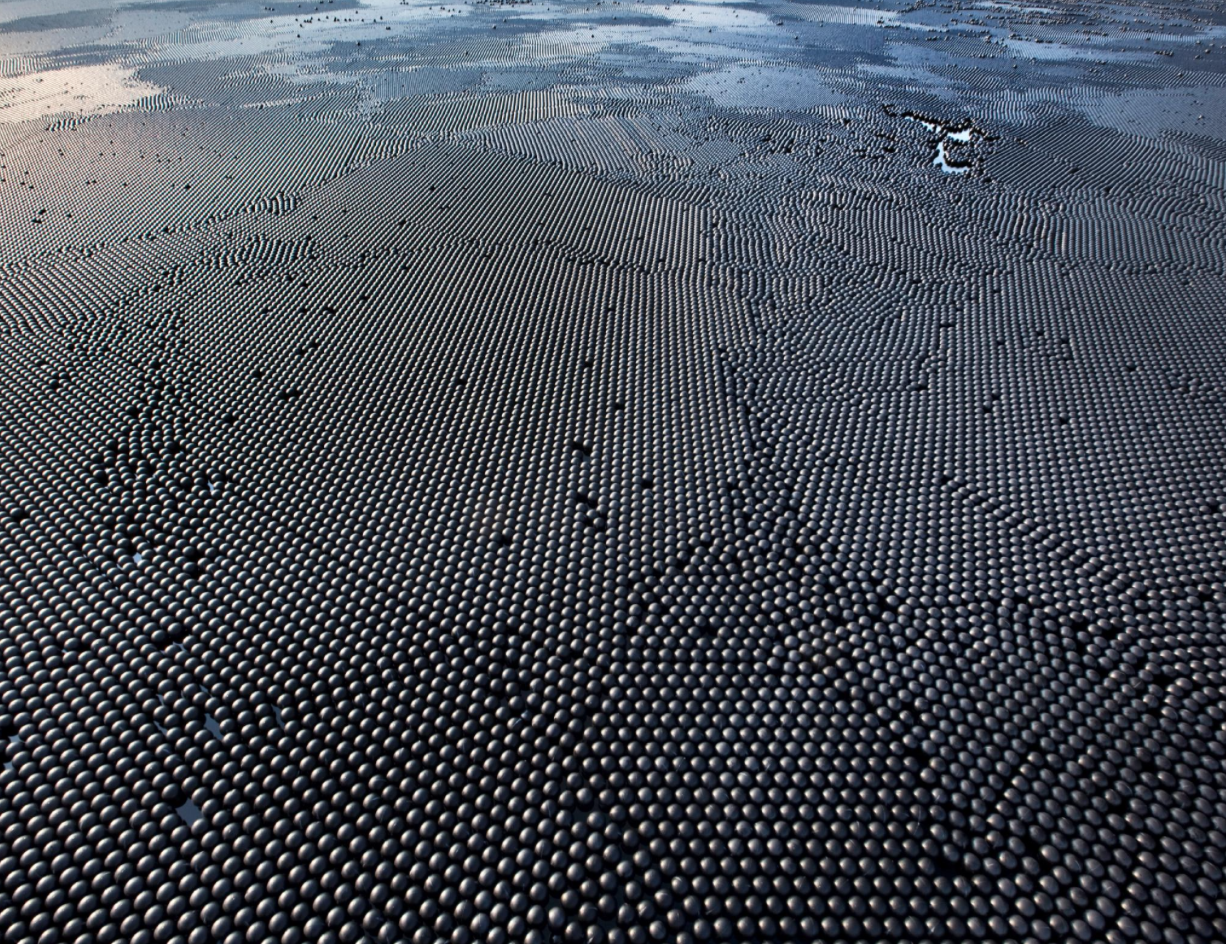
\includegraphics[width=\linewidth]{shade-balls}
  \caption[Shade balls in Los Angeles]{
    Shade balls covering the Los Angeles reservoir to prevent water evaporation.
    These balls spontaneously form long-range hexagonal ordering, reminiscent of crystallisation in atomic systems.
    As macroscopic objects these balls interact primarily as hard spheres.
    Image by Gerd Ludwig, \emph{National Geographic} (2007).}
  \label{fig:shade-balls}
\end{SCfigure}

Despite their coarse simplification of real atomic interactions, we see that hard spheres actually capture a lot of the essential physics.
To illustrate this consider the phase diagram of hard spheres Figure \ref{fig:hs-phase-diagram}.
We see there is a freezing transition at $\eta = 0.494$, suggesting that the liquid will spontaneously order into a crystal at high densities.
This is surprising, in everyday scenarios (e.g.\ water) we are used to seeing crystallisation as one lowers temperature and the explanation normally given in classrooms is that the crystal is favoured due to attractions between molecules.
Now, in real systems crystallisation can also be triggered by changes to density also so density being a control parameter is not a problem, however the lack of attractions should, if this intuition were correct, prohibit crystallisation.

It turns out in the case of hard spheres that the crystal has a larger entropy above freezing, so entropy itself triggers crystallisation.
This was a hotly debated topic \cite{?,?,?} until is was solved by computer simulation in \cite{?,?,?} and experiment \cite{?,?,?}.
Part of the reason people could not believe that the crystal is entropically favoured, is because we often mistakenly take entropy to be a measure of disorder when it in fact more complicated.
The crystal might be more ordered than the liquid, with a lower \emph{configurational} entropy, however the entropy includes \emph{all} microstates not just averaged ones: the crystal is compensated by having a much larger \emph{vibrational} entropy than the liquid at high densities.
Including both these contributions leads to the phase diagram that we know today.

A similar effect is seen in balls floating on water as in e.g.\ peas in a saucepan or shade balls covering a reservoir.
The hard interactions between the balls causes%
\marginfootnote{In an attempt to find an everyday example, I have taken liberties with the interaction being purely hard; I suspect that floating balls feature effective attractions due to \emph{hydrodynamic} interactions at the water surface.}[-3cm]
them to `crystallise' at high densities as seen in Figure \ref{fig:shade-balls}..
Strictly speaking these are not crystals in the sense of long-range \emph{translational} order, instead they are said to possess long-range \emph{orientational} order.
This subtlety emerges because the floating balls are confined to the water surface making them effectively two dimensional; fluctuations are strong enough in two dimensions to overcome truly long-ranged positional ordering \cite{MerminPRL1966,MerminPR1968}.

We have extolled the virtues of hard spheres, however this should not be interpretted as saying that this model system capture \emph{all} of the physics of real systems: it is a toy system after all.
They are merely a very good starting point for more complex systems.
As an example of physics they do \emph{not} capture, consider the critical point of real liquids.
Liquid-gas critical phenomena emerges from a competition between attractive and repulsive forces, with divergent fluctuations at the critical point.
It is thus impossible for a system with purely repulsive interactions, like hard spheres, to feature a critical point.
That being said, many theories predict critical phenomena quite well by taking a hard sphere potential and incorporating a mean-field like attractive perturbation \cite{?} so a hard sphere system provides a good reference point.

Hard spheres exist in more than just a theorist's imagination: they can be experimentally realised in colloidal experiments.
Colloidal suspensions are mixtures of solute immersed in a solvent composed of much smaller particles.
Colloidal particles are typically at the micron-scale.
These typically feature complex interactions \cite{Royall?,?,?} however these can be tailored to closely approximate hard sphere like interactions through steric stabilisation.
\todo{What is an aerosol? What is a dispersion?}
Colloidal experiments closely match hard simulations and theoretical predicitons \cite{?}.
Notably one can determine the phase diagram see Figure \ref{fig:hs-phase-diagram}.
Note the glass at very high densities.

\begin{SCfigure}
  \missingfigure[figwidth=\linewidth]{}%
  \caption[The hard sphere phase diagram]{
    The hard sphere phase diagram, including the metastable branch.
    a: theoretical phase diagram.
    b: experiments, including the glass (image reproduced from \cite{?}).
    This is one of the most iconic images in the field, and no discussion of colloidal hard spheres would be complete without it.}
  \label{fig:hs-phase-diagram}
\end{SCfigure}

\begin{SCfigure}
  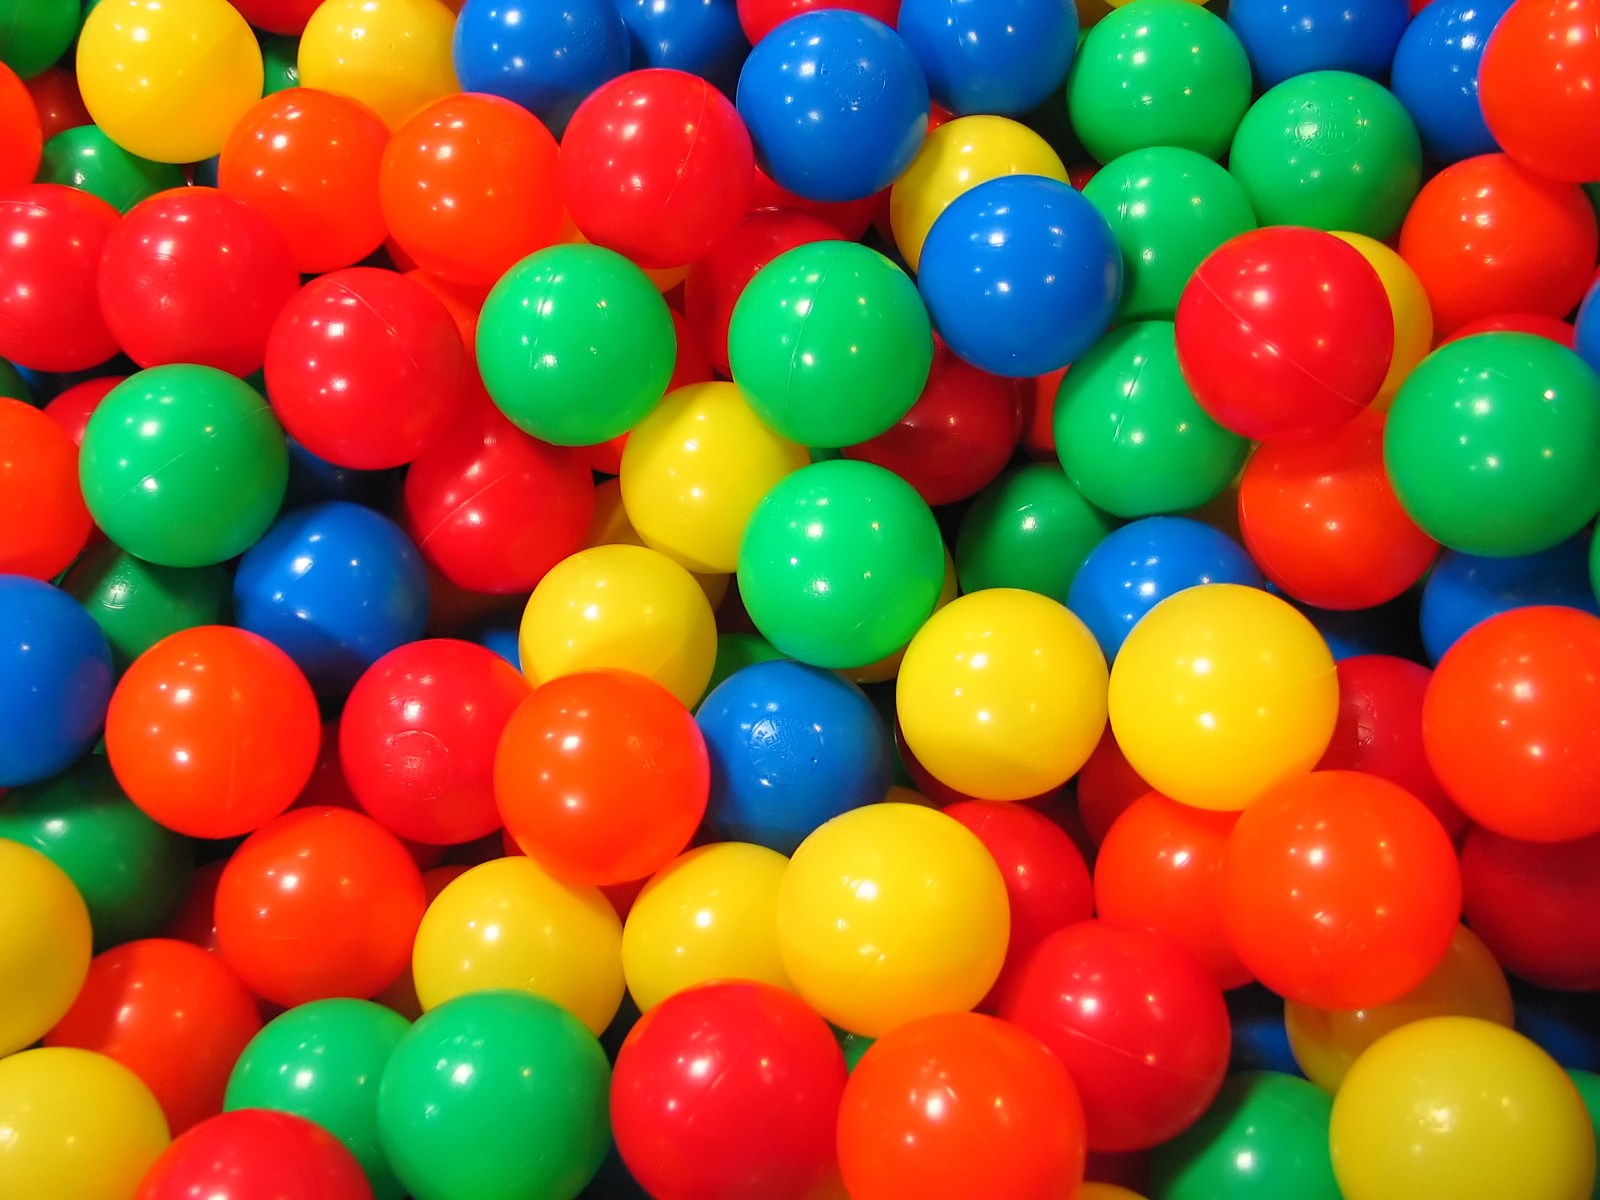
\includegraphics[width=\linewidth]{ball-pit-horizontal}
  \caption[Random close packing in a ball pit]{
    Random close packing of hard spheres in a ball bit.
    Image by Peter Ong.}
  \label{fig:rcp}
\end{SCfigure}

\begin{SCfigure}
  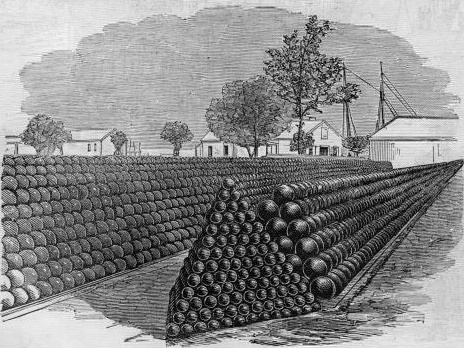
\includegraphics[width=\linewidth]{cannonballs}
  %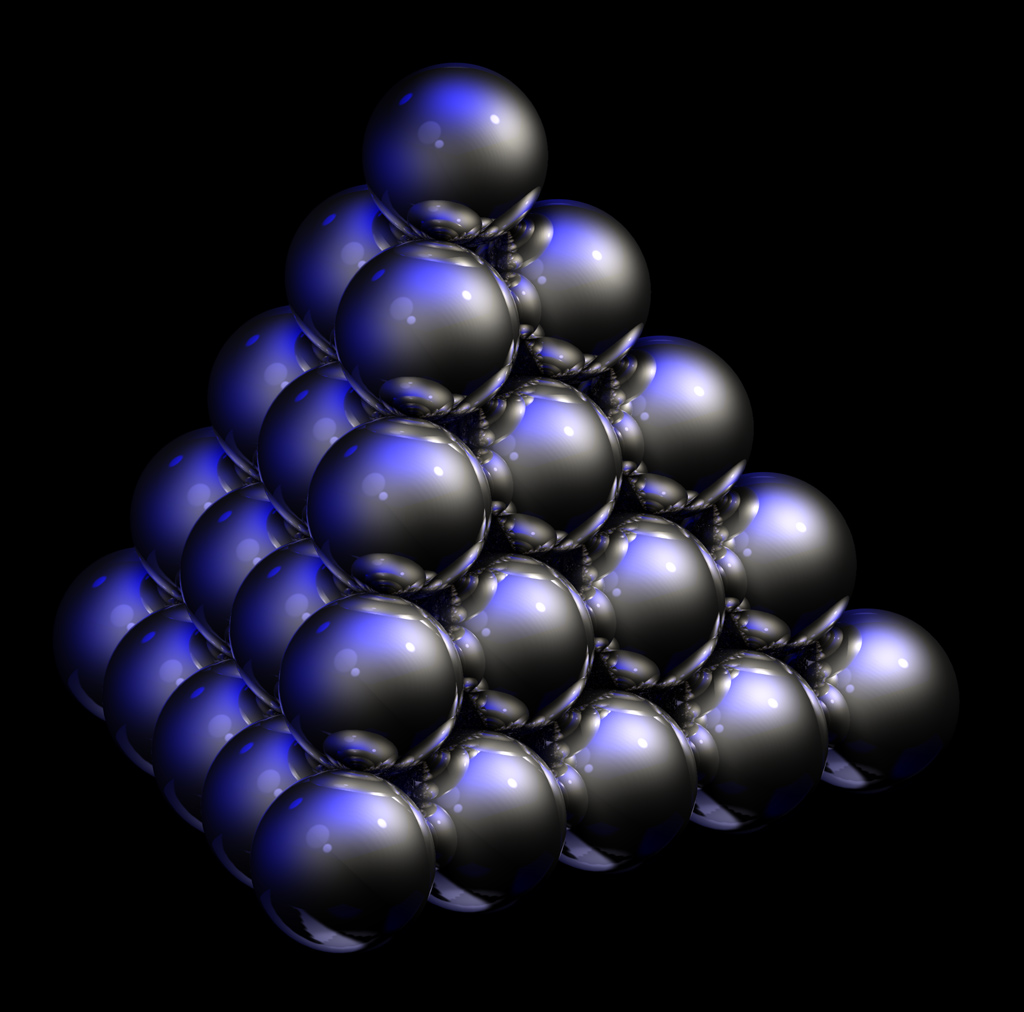
\includegraphics[width=\linewidth]{close-packed-spheres}
  \caption[Close packed cannonballs]{
    Sketch of close-packed stacks of cannonballs in Fortress Monroe.
    Image by Stacy, \emph{Harper's weekly} (1861)}
  \label{fig:fcc}
\end{SCfigure}

As the most widely studied model interaction potential we know a lot about its equilibrium structure (phase diagram) in bulk and even inhomogeneous thanks to density functional theory \cite{?,?,?}.
However, its behaviour off-equilibrium at high densities is hotly debated.
The two biggest unresolved research topics for this subject:
\begin{itemize}
\item \emph{Nucleation}: given that above freezing the crystal ? Theoretically predicted nucleation rates from simulation studies differ by 12 orders of magnitudes from experiments, purported to be the second biggest disagreement between theory and experiment in all of science \cite{?}.
\item \emph{Metastable liquid}: if one could avoid crystallisation and equilibrate only over the liquid microstates, what would be the ultimate fate of the liquid?
  We will talk more about this in \ref{?}.
\end{itemize}

There is a deep connection between hard spheres and computer science.
Packing problems have been studied \cite{Cohn,Conway,Sloane} and they are notoriously difficult; Kepler conjectured the optimal packing in 3d was the face-centred cubic/hexagonal close packing but it took 300(?check) years to solve this.
The final proof was computer aided, and not simple.
Packing problems are connected with encoding/encryption.
Transmitting a signal requires a way to encode a message across a band(?): if packed too tightly on the band(?) then noise will destroy the signal to it is desirable to optimise the sites for bits \cite{Cohn,?,?}.
Additionally, lattice based encryption techniques are one of the alternatives to prime factorisation: the coming development of quantum computers \cite{?,?} would render prime factorisation easy because of Shor's algorithm \cite{Shor?} rendering standard encryption techniques insecure.
The techniques developed for the mean field hard sphere problem have been applied to the perceptron model \cite{?}, and deep-learning neural networks which are naturally high dimensional problems lending themselves to a mean field treatment \cite{?}.

Although hard spheres will be our focus, we will mention the importance of systems of hard particles of other shapes for self-assembly.
Self-assembly is an active area of soft matter: it is technologically desirable to tailor the final structure by controlling the building blocks.
Imagine assembling nanomachines or artificial cells by controlling the chemistry.
It is found that varying the size and shape of hard particles can reproduce all the complexity of the periodic table \cite{Glotzer?,Dijkstra?}.
Hard spheres are the simplest such system, so a theory which can treat other geometries is desirable.

The primary goal of this thesis is to advance the methods of treating liquids at high densities, particularly concerning the role of thermodynamics in dynamical arrest and nucleation.
These methods can be readily adapted to more complex systems, such as protein folding in aqueous solution or self-assembly of complex structures.

A secondary goal would be to advance the understanding of the fundamental theory of hard particles in some small way.
I have attempted to develop the geometrical theory behind the methods of Chapters \ref{?} and \ref{?} in a generally applicable way;
I have done this to the best of my ability, but my primary skills lie in numerical methods and I am a second-rate theoretician.

\section{Supercooled liquids and glasses}

It is widely reported that glass is actually liquid, and as evidence of this the thickness of old windows at the bottom is pointed to.
This is actually a matter of some dispute, but contains a grain of truth.
Pre-modern methods of creating window glass involved spinning molten glass on magma to flatten it out.
Centrifugal forces caused the glass to be thicker on the outer disk, so panes of glass would always be heavier in one direction%
\marginfootnote{And personally, if I were setting an uneven pane of glass I would place the heavy part at the bottom.}.

To a soft matter physicist glass is a broader term, referring to a wide class of materials while the window glass of common parlance is referred to by its chemical name \emph{silicate}.
This class of materials share many features of being disordered etc \cite{?} although in some sense they are connected by what they do \emph{not} do: which is flow on human timescales.
When I refer to `glass' I will be using it in this broad technical sense of a state of matter.
Some examples besides silicate:
\begin{itemize}
\item Most of the ice in the universe exists in an amorphous state in comets \cite{?}
\item Ceramics
\item Plastics: amorphous polymers
\end{itemize}
Of more abstract nature which could be called glassy though they are not materials
\begin{itemize}
\item Gels: super glasses, liquid like bit plus a network/backbone which has glassy dynamics
\item Neural networks
\item Non-deterministic polynomial time (NP) problems
\end{itemize}
We will not be directly addressing the latter type of more abstract problems which could be considered glasses, although they are arguably related due to a similar underlying disorder.
We will be focusing on only the most rudimentary of glassy phenomenology: the dynamical arrest of liquids at high densities/low temperatures when crystallisation is avoided.
Especially as it manifests in hard spheres, which as discussed is the reference system of choice for simple liquids.

So what do we mean by dynamical arrest.
Typically we can look at one of two (related) quantities: viscosity or relaxation time.
Viscosity measures how resistant the thing is to flow, while relaxation time measures the typical microscopic time for things to move around i.e.\ liquid like behaviour.
As a practical definition, a glass is defined in the lab as any material for which the relaxation time exceeds 100\ce{s}: this point is called the experimental glass transition.
This is somewhat arbitrary, although the location of the glass transition point is not particularly sensitive to where you set the threshold because of how rapidly the viscosity/times are increasing around there.
\todo{Need: Angell plot, fragile vs strong}

Personally, the observation that got me interested in the field is the entropy argument.
If one compares the difference between the entropy of the crystal and the glass, and extrapolates wildly one expects there to be a point where the glass has a lower entropy than the crystal.
This is not very meaningful by itself, as we have already established by discussing the crystal vibrational entropy can be quite subtle so it is possible for the liquid to have a lower vibrational entropy.
However, if one corrects this with more modern techniques to measure just the entropy corresponding to non-trivial motion we see that there is a point where the configurational (i.e.\ not purely vibrational) entropy vanishes: this would imply the system is frozen in a single configuration.
Such a point would define a transition to a genuine thermodynamic phase, an ideal glass.
\todo{Plots of configurational entropy}

A diverging timescale necessarily requires a diverging point-to-set length scale and a vanishing configurational entropy, a proof given in \cite{?}.
This must trivially occur at the very least $T=0\si{K}$ where relaxation timescales diverges, however much like the lack of a phase transition in the Ising model in $d=1$ this is not a true thermodynamic phase transition because it cannot be crossed.
Recent numerical evidence suggests that a model glassformer in $d=2$ does not show a transition, also vanishing at $T=0\si{K}$ \cite{Berthier?}.
So the central question of glass is what happens in $d=3$, is there a vanishing configurational entropy at a finite $T > 0$ with an accompanying thermodynamic glass transition?
In mean-field, formally in the limit of infinite spatial dimensions $d \to \infty$, the hard sphere system has been shown to have a true transition, however the critical dimensions are unknown so it is unclear what happens in $d=3$ \cite{Parisi,Zamboni,Charbonneau,Kurchan,?,?}.

\todo{Jamming: how does it relate to glass}

\section{Notes from Tarjus}

Overview of the glass transition.
Salient features: why hard, interesting, unique.

What is a glass?
Frozen in a (apparently) disordered state.
All sorts of glasses, structural, spin, orientational, electron, vortex.
Glasses formed by liquids, colloidal suspensions and polymers: traditional structural glasses.
Solid: doesn't flow on observational time, resists small/infinitesimal shear (acts like solid).
Amorphous, apparently amorphous: no periodic arrangement like in crystal.
Homogeneous makes useful for technology: useful for e.g.\ optical properties.

Hard glasses: high elastic constants.
Colloidal suspensions: soft matter version, small elastic constants.
Same phenomenology though.

Cooling a liquid.
Take thermodynamic quantity (e.g.\ volume, entropy, enthalpy): usually crystallise.
(Picture)
First-order transition bypassed by quick cooling.
Enter supercooled liquid phase.
No longer equilibrates/relax/flows, call it a glass: occurs at glass transition.
Glass is a solid for all practical purposes.

SC liquid: same characteristics as at equilibrium.
Independent of preparation: loses memory of initial preparation.
Measureable properties have time translational invariance/are stationary.
Time independence of all observables, i.e.\
\begin{equation}
  \langle A(t) \rangle = \langle A \rangle
\end{equation}
including correlation functions e.g.\
\begin{equation}
  \langle A(t) A(t') \rangle = \langle A(0) A(t - t') \rangle
\end{equation}
(equation for stationary)
Fluctuation-dissipation theorems.
Linear response regime: response to perturbation related to correlation function (spontaneous fluctuations).
\begin{equation}
  \chi_A (t, t')
  =
  - \beta \Theta(t - t')
  \frac{d}{dt}
  \left(
  \bigg\langle
  (A(t) - \langle A \rangle)
  (A(0) - \langle A \rangle)
  \bigg\rangle
  \right)
\end{equation}

\ifdefined\includebibliography
  \printbibliography
\fi
  
\end{document}
